% \documentclass{article}

% % Recommended, but optional, packages for figures and better typesetting:
% \usepackage{microtype}
% \usepackage{graphicx}
% % \usepackage{subfigure}
% \usepackage{booktabs} % for professional tables
% \usepackage{subcaption}
% \usepackage[noend]{algpseudocode}
% \usepackage{enumitem}
% \usepackage{amsmath}
% \usepackage{amssymb}

% % hyperref makes hyperlinks in the resulting PDF.
% % If your build breaks (sometimes temporarily if a hyperlink spans a page)
% % please comment out the following usepackage line and replace
% % \usepackage{icml2021} with \usepackage[nohyperref]{icml2021} above.
% \usepackage{hyperref}

% % Attempt to make hyperref and algorithmic work together better:
% \newcommand{\theHalgorithm}{\arabic{algorithm}}
% \usepackage{multirow}

% % Use the following line for the initial blind version submitted for review:
% \usepackage{icml2021}
% % operators

% \newcommand{\argmax}{\operatornamewithlimits{argmax}}
% \newcommand{\argmin}{\operatornamewithlimits{argmin}}

% vectors
\let\avec\vec
%\renewcommand{\vec}[1]{\ensuremath{\boldsymbol{#1}}}
\renewcommand{\v}[1]{\ensuremath{\boldsymbol{#1}}}

\newcommand{\src}{\lstinline[mathescape, keepspaces]}
\newcommand{\msrc}[1]{\mbox{\src!#1!}}

% \newcommand{\tens}[1]{%
%   \mathbin{\mathop{\otimes}\limits_{#1}}%
% }

% symbol shorthands (lowercase)
\newcommand{\x}{\ensuremath{\v{x}}}
\newcommand{\y}{\ensuremath{\v{y}}}
\newcommand{\z}{\ensuremath{\v{z}}}
\newcommand{\h}{\v{\eta}}
\newcommand{\e}{\v{\epsilon}}
\renewcommand{\u}{\v{u}}
\newcommand{\pd}{\ensuremath{\partial}}
% \newcommand{\x}{\ensuremath{x}}
% \newcommand{\y}{\ensuremath{y}}
% \newcommand{\z}{\ensuremath{z}}
% \newcommand{\h}{\ensuremath{\eta}}
% \newcommand{\e}{\ensuremath{\epsilon}}
\renewcommand{\u}{\ensuremath{u}}
\newcommand{\q}{\theta}
\newcommand{\f}{\phi}
\renewcommand{\l}{\lambda}
\renewcommand{\t}{\tau}

% symbol shorthands (uppercase)
\renewcommand{\L}{\ensuremath{\mathcal{L}}}
% \newcommand{\KL}[2]{\ensuremath{\mathrm{KL}\left({#1} \:\middle\vert\middle\vert\: {#2}\right)}}
\newcommand{\E}{\ensuremath{\mathbb{E}}}
\newcommand{\N}{\ensuremath{\mathcal{N}}}
\newcommand{\C}{\ensuremath{\mathtt{Concrete}}}

%\let\lmid\mid
%\renewcommand{\mid}{\!\lmid\!}

\newcommand{\eval}{\ensuremath{$\reflectbox{$\,\leadsto\,$}$}}
%\newcommand{\eval}{\sim}
\newcommand{\hide}[1]{}

\makeatletter
\DeclareRobustCommand{\cev}[1]{%
  \mathpalette\do@cev{#1}%
}
\newcommand{\do@cev}[2]{%
  \fix@cev{#1}{+}%
  \reflectbox{$\m@th#1\vec{\reflectbox{$\fix@cev{#1}{-}\m@th#1#2\fix@cev{#1}{+}$}}$}%
  \fix@cev{#1}{-}%
}
\newcommand{\fix@cev}[2]{%
  \ifx#1\displaystyle
    \mkern#23mu
  \else
    \ifx#1\textstyle
      \mkern#23mu
    \else
      \ifx#1\scriptstyle
        \mkern#22mu
      \else
        \mkern#22mu
      \fi
    \fi
  \fi
}

% % If accepted, instead use the following line for the camera-ready submission:
% %\usepackage[accepted]{icml2021}

% % The \icmltitle you define below is probably too long as a header.
% % Therefore, a short form for the running title is supplied here:
% \icmltitlerunning{Supplementary Materials}

% \begin{document}
\newpage
\onecolumn
\icmltitle{Supplementary Materials for Conjugate Energy-Based Models}
\appendix

\section{Connection to Other Models}
\label{app:sec:connection-to-other-models}

\subsection{VAEs}
\label{app:sec:vae}
We can interpret the generative model in a VAE as a model with an energy function
\begin{align}
    E_\q(x, z) = -t(x)^\top \eta_\q(z) - b_\q(z), \qquad \eta_\q(z) = \eta(\mu_\q(z)).
\end{align}
In this setting, $\mu_\q(z)$ is the generator network that maps low-dimensional latent variables to a high-dimensional vector of natural parameters. The function $t(x)$ is a known mapping of data to the sufficient statistics of a Gaussian or Bernoulli likelihood.

The bias $b_\q(z)$ contains the terms in the log density $\log p_\q(x,z)$ that only depend on $z$. There are two such terms: (1) the log prior $\log p(z)$, (2) the log normalizer $A(\eta_\q(z))$ for the likelihood $\log p_\q(x \mid z)$.  Combining these terms yields the bias
% Given that the two most common likelihoods in VAEs are the Gaussian and Bernoulli distributions, which can be computed in closed form because  are in the exponential family.
\begin{align}
    \label{eq:vae-bias}
    b_\q(z) = \log p(z) - A(\eta_\q(z)).
\end{align}
In other words, in a VAE we use known sufficient statistics $t(x)$, and train a generator to learn the natural parameters $\eta_\theta(z)$. In a CEBM, by contrast, we assume known natural parameters $\eta(z)$ and train an encoder to learn the sufficient statistics $t_\theta(x)$. It is worth noting that this formulation only applies when the VAE's likelihood satisfies two conditions: (1) it belongs to an exponential family (2) the base measure does not depend on $x$.   


\subsection{Exponential Family Harmoniums}
\label{app:sec:rbm}

There is a long history of incorporating latent variables in EBMs, particularly in the context of restricted Boltzmann machines (RBMs)~\citep{smolensky1986information,hinton2002training}, deep belief nets~\citep{hinton2006fast}, and deep Boltzmann machines~\citep{salakhutdinov2009deep}. The idea of formulating EBMs into the exponential family is also not new; \citet{welling2005exponential} proposed a new class of models called Exponential Family Harmoniums (EFHs) by extending RBMs into the exponential family. In this Section, we discuss the connection between our approach to these models. Concretely, we show that EFHs can be recovered a special case of CEBMs.

For observed variable $x$ and latent variable $z$, the energy of an RBM is defined as
\begin{align}
    \label{eq:rbm}
    E^{\text{RBM}}_{\q}(x,z)
    = -x^\top\theta_{xz}z - \theta_x^{\top}x - \theta_z^{\top}z,
\end{align}
where $\theta_x \in \mathbb{R}^D$, $\theta_z \in \mathbb{R}^K$, and $\theta_{xz} \in \mathbb{R}^{D \times K}$. In RBMs, the conditional distributions $p_{\q}(x|z)$ and $p_{\q}(z|x)$ are both tractable which means that during constitutive divergence, we can sample $x \sim p_\q(x)$ using Gibbs sampling.

EFHs extend these models into the exponential family by incorporating the sufficient statistics of $x$ and $z$ in the energy,
\begin{align}
    \label{eq:efh}
    E^{\text{EFH}}_{\q}(x,z)
    = -t_x(x)^\top\theta_{xz}t_z(z) - \theta_x^{\top}t_x(x) - \theta_z^{\top}t_z(z),
\end{align}
where $t_x(\cdot)$ and $t_z(\cdot)$ are the sufficient statistics for variables $x$ and $z$ respectively. \citet{welling2005exponential} show that this energy function yields the following conditional distributions:
\begin{align}
    \label{eq:efh-conditional}
    \text{Likelihood} \qquad p_{\q}(x|z) &= \exp \left\{ t_x(x)^{\top}\tilde{\q}_x - A_x(\tilde{\q}_x)\right\}, \qquad \tilde{\q}_x = \q_x + \theta_{xz}t_z(z), \\
    \text{Posterior} \qquad p_{\q}(z|x) &= \exp \left\{ t_z(z)^{\top}\tilde{\q}_z - A_z(\tilde{\q}_z)\right\}, \qquad \tilde{\q}_z = \q_z + \theta_{xz}t_x(x),
\end{align}
where $\tilde{\q}_x$ and $\tilde{\q}_z$ are the canonical parameters, and $A_x(\cdot)$ and $A_z(\cdot)$ are the log normalizer of the models $p_{\q}(x|z)$ and $p_{\q}(z|x)$ respectively. Given that both conditional distributions are tractable, EFHs have the same advantage as RBMs: We can use a Gibbs sampler for sampling $x$. 


% exponential family
Our work can be considered an extension of EFHs; If we set
\begin{align}
    t_{\q}(x)=[t_x(x)^\top\theta_{xz},\ t_x(x)^\top\theta_{x}], \qquad \eta(z)=[t_z(z),\ 1], \qquad b_{\q}(z)=t_z(z)^\top\theta_{z},
\end{align}
in Equation~\ref{eq:cebm-energy}, we recover the energy function for an EFH. Perhaps the most crucial difference between CEBMs and EFHs (and other RBM-based models) is the non-linearity relationship between the observed and latent variables. The non-linearity in $t_{\q}(\cdot)$ has the benefit of providing the flexibility to learn more complex structures in the data. This modelling choice however comes with a cost. In CEBMs, while the posterior is still tractable, the likelihood model is not. As a consequence, we lose the ability to use Gibbs sampling to sample $x \sim p_\q(x)$. However, given that our motivation here is not to generate high quality samples at test time but to learn good representations representations, we believe giving up the ability to easily sample $x$ in order to learn more complex structures while keeping the posterior tractable is an appropriate trade-off.  
 
% In other words, only one of the conditional distributions (the posterior) is tractable.

\section{Derivation of Prior and Likelihood in a CEBM}
\label{app:sec:derivations}

\subsection{Prior}

\begin{align}
    p_{\q}(z) 
    &=  \int \!dx \: \frac{1}{Z_\q}\exp \{- E_\q(x,z)\} \\
    &= \frac{1}{Z_\q} \int \!dx \: \exp \{- E_\q(x,z)\} \\
    &= \frac{1}{Z_\q} \int \!dx \: \exp \{t_\q(x)^{\top}\eta(z) + b(z)\} \\
    &= \frac{\exp\{b(z)\}}{Z_\q} \int \!dx \: \exp \{t_\q(x)^{\top}\eta(z)\}
\end{align}

\subsection{Likelihood}

\begin{align}
    p_{\q}(x|z) 
    &= \frac{p_{\q}(x,z)}{p_{\q}(z)} \\
    &= \frac{\frac{1}{Z_\q}\exp \{- E_\q(x,z)\} }{\frac{\exp\{b(z)\}}{Z_\q} \int \!dx \: \exp \{t_\q(x)^{\top}\eta(z)\}} \\
    &= \frac{\frac{\exp\{b(z)\}}{Z_\q} \exp \{t_\q(x)^{\top}\eta(z)\} }{\frac{\exp\{b(z)\}}{Z_\q} \int \!dx \: \exp \{t_\q(x)^{\top}\eta(z)\}} \\
    &= \frac{\exp \{t_\q(x)^{\top}\eta(z)\} }{\int \!dx \: \exp \{t_\q(x)^{\top}\eta(z)\}}
\end{align}



\section{Model Architectures}
\label{appendix-architectures}
Table~\ref{appendex:tab:arch-cebm}, Table~\ref{appendex:tab:arch-vae}, and Table~\ref{appendex:tab:arch-igebm} show the architectures used for CEBM, VAE, and IGEBM, respectively.

\begin{table}[!h]
\caption{Architecture of CEBM}
    \centering
    \begin{subtable}[h]{.5\linewidth}
    \caption{MNIST and Fashion-MNIST.}
    \centering
        \begin{tabular}{|l|}
        \toprule
        \textbf{Encoder} \\
        \midrule
        Input $28\times28\times1$ images  \\
        \hline 
        $3\times3$ conv. 64 LeakyReLU. stride 1. padding 1  \\
        \hline 
        $4\times4$ conv. 64 LeakyReLU. stride 2. padding 1 \\
        \hline 
        $4\times4$ conv. 32 LeakyReLU. stride 2. padding 1  \\
        \hline
        $4\times4$ conv. 32 LeakyReLU. stride 2. padding 1 \\
        \hline
        FC. 128 LeakyReLU \\
        \hline
        FC. $2\times128$ \\
        \bottomrule
        \end{tabular}
    \end{subtable}%%%
    \begin{subtable}[h]{.5\textwidth}
    \caption{CIFAR10 and SVHN.}
    \centering
        \begin{tabular}{|l|}
        \toprule
        \textbf{Encoder}  \\
        \midrule
        Input $32\times32\times3$ images  \\
        \hline 
        $3\times3$ conv. 64 LeakyReLU. stride 1. padding 1  \\
        \hline 
        $4\times4$ conv. 128 LeakyReLU. stride 2. padding 1 \\
        \hline 
        $4\times4$ conv. 256 LeakyReLU. stride 2. padding 1  \\
        \hline
        $4\times4$ conv. 512 LeakyReLU. stride 2. padding 1  \\
        \hline
        FC. 128 LeakyReLU \\
        \hline
        FC. $2\times128$\\
        \bottomrule
        \end{tabular}
    \vspace*{1ex}
    \end{subtable}
    \label{appendex:tab:arch-cebm}
\end{table}



% \newpage
\begin{table}[!h]
\caption{Architecture of VAE}
    \centering
    \begin{subtable}[h]{\textwidth}
    \caption{MNIST and Fashion-MNIST.}
    \centering
        \begin{tabular}{|l|l|}
        \toprule
        \textbf{Encoder} & \textbf{Decoder} \\
        \midrule
        Input $28\times28\times1$ images & Input $z\in \mathbb{R}^{128}$ latent variables \\
        \hline 
        $3\times3$ conv. 64 LeakyReLU. stride 1. padding 1 & FC. 128 ReLU \\
        \hline 
        $4\times4$ conv. 64 LeakyReLU. stride 2. padding 1 & FC. $3\times3\times32$ ReLU \\
        \hline 
        $4\times4$ conv. 32 LeakyReLU. stride 2. padding 1 & $4\times4$ upconv. 32 LeakyReLU. stride 2. padding 1 \\
        \hline
        $4\times4$ conv. 32 LeakyReLU. stride 2. padding 1 & $4\times4$ upconv. 64 LeakyReLU. stride 2. padding 1 \\
        \hline
        FC. 128 ReLU & $4\times4$ upconv. 64 LeakyReLU. stride 2. padding 0 \\
        \hline
        FC. $2\times128$ & $3\times3$ upconv. 1 stride 1. padding 0 \\
        \bottomrule
        \end{tabular}
    \vspace*{1ex}
    \end{subtable}
    \begin{subtable}[h]{\textwidth}
    \caption{CIFAR10 and SVHN.}
    \centering
        \begin{tabular}{|l|l|}
        \toprule
        \textbf{Encoder} & \textbf{Decoder} \\
        \midrule
        Input $32\times32\times3$ images & Input $z\in \mathbb{R}^{128}$ latent variables \\
        \hline 
        $3\times3$ conv. 64 LeakyReLU. stride 1. padding 1 & FC. 128 ReLU \\
        \hline 
        $4\times4$ conv. 128 LeakyReLU. stride 2. padding 1 & FC. $4\times4\times512$ ReLU \\
        \hline 
        $4\times4$ conv. 256 LeakyReLU. stride 2. padding 1 & $4\times4$ upconv. 32 LeakyReLU. stride 2. padding 1 \\
        \hline
        $4\times4$ conv. 512 LeakyReLU. stride 2. padding 1 & $4\times4$ upconv. 64 LeakyReLU. stride 2. padding 1 \\
        \hline
        FC. 128 ReLU & $3\times3$ upconv. 64 LeakyReLU. stride 2. padding 1 \\
        \hline
        FC. $2\times128$ & $3\times3$ upconv. 1 stride 1. padding 1 \\
        \bottomrule
        \end{tabular}
    \vspace*{1ex}
    \end{subtable}
    \label{appendex:tab:arch-vae}
\end{table}

\begin{table}[!h]
\caption{Architecture of IGEBM}
    \centering
    \begin{subtable}[h]{.5\textwidth}
    \caption{MNIST and Fashion-MNIST.}
    \centering
        \begin{tabular}{|l|}
        \toprule
        \textbf{Encoder} \\
        \midrule
        Input $28\times28\times1$ images  \\
        \hline 
        $3\times3$ conv. 64 LeakyReLU. stride 1. padding 1  \\
        \hline 
        $4\times4$ conv. 64 LeakyReLU. stride 2. padding 1 \\
        \hline 
        $4\times4$ conv. 32 LeakyReLU. stride 2. padding 1  \\
        \hline
        $4\times4$ conv. 32 LeakyReLU. stride 2. padding 1 \\
        \hline
        FC. 128 LeakyReLU \\
        \hline
        FC. 128 LeakyReLU. FC. 1 \\
        \bottomrule
        \end{tabular}
    \end{subtable}%%%
    \begin{subtable}[h]{.5\textwidth}
    \caption{CIFAR10 and SVHN.}
    \centering
        \begin{tabular}{|l|}
        \toprule
        \textbf{Encoder}  \\
        \midrule
        Input $32\times32\times3$ images  \\
        \hline 
        $3\times3$ conv. 64 LeakyReLU. stride 1. padding 1  \\
        \hline 
        $4\times4$ conv. 128 LeakyReLU. stride 2. padding 1 \\
        \hline 
        $4\times4$ conv. 256 LeakyReLU. stride 2. padding 1  \\
        \hline
        $4\times4$ conv. 512 LeakyReLU. stride 2. padding 1  \\
        \hline
        FC. 128 LeakyReLU \\
        \hline
        FC. 128 LeakyReLU. FC. 1\\
        \bottomrule
        \end{tabular}
    \vspace*{1ex}
    \end{subtable}
    \label{appendex:tab:arch-igebm}
\end{table}

\section{Training Details}
\label{app:sec:training-details}
In CEBMs and VAEs, we choose the dimension of latent variables to be 128. For CEBMS, We found that the optimization becomes difficult with smaller dimensions. We L2 regularize energy magnitudes (proposed by~\citet{du2019implicit}), where the coefficient of the L2 regularization term is 0.1. We empirically found that the training would become unstable without this regularization. We train our models using 60 SGLD steps where we initialize samples from the replay buffer with 0.95 probability, and initialize from uniform noise with 0.05 probability. We train all the models with 90k gradient steps, batch size 128, Adam optimizer with learning rate 1e-4. When doing PCD, we used a reply buffer of size 5000. We set the $\alpha$ in the SGLD teps to be 0.075. Similar to~\citet{du2019implicit}, we found it useful to add some noise to the image before encoding. In our experiments, we used Gaussian noise with $\sigma^{2} = 0.03$. For the mixture models (CEBMM and GMM-VAE), we used 50 mixtures.  

\newpage
\section{Additional Results}
\label{app:sec:additional-results}

\subsection{Confusion Matrices on 1-NN Classification}
\label{appendix-sec:confuion matrices}
We perform 1-nearest-neighbor classification task for MNIST, Fashion-MNIST, SVHN, CIFAR10. We compute the L2 distance in the latent space of VAE, IGEBM and CEBM, and also in pixel space. We visualize the confusion matrices
\begin{figure}[!h]
\centering
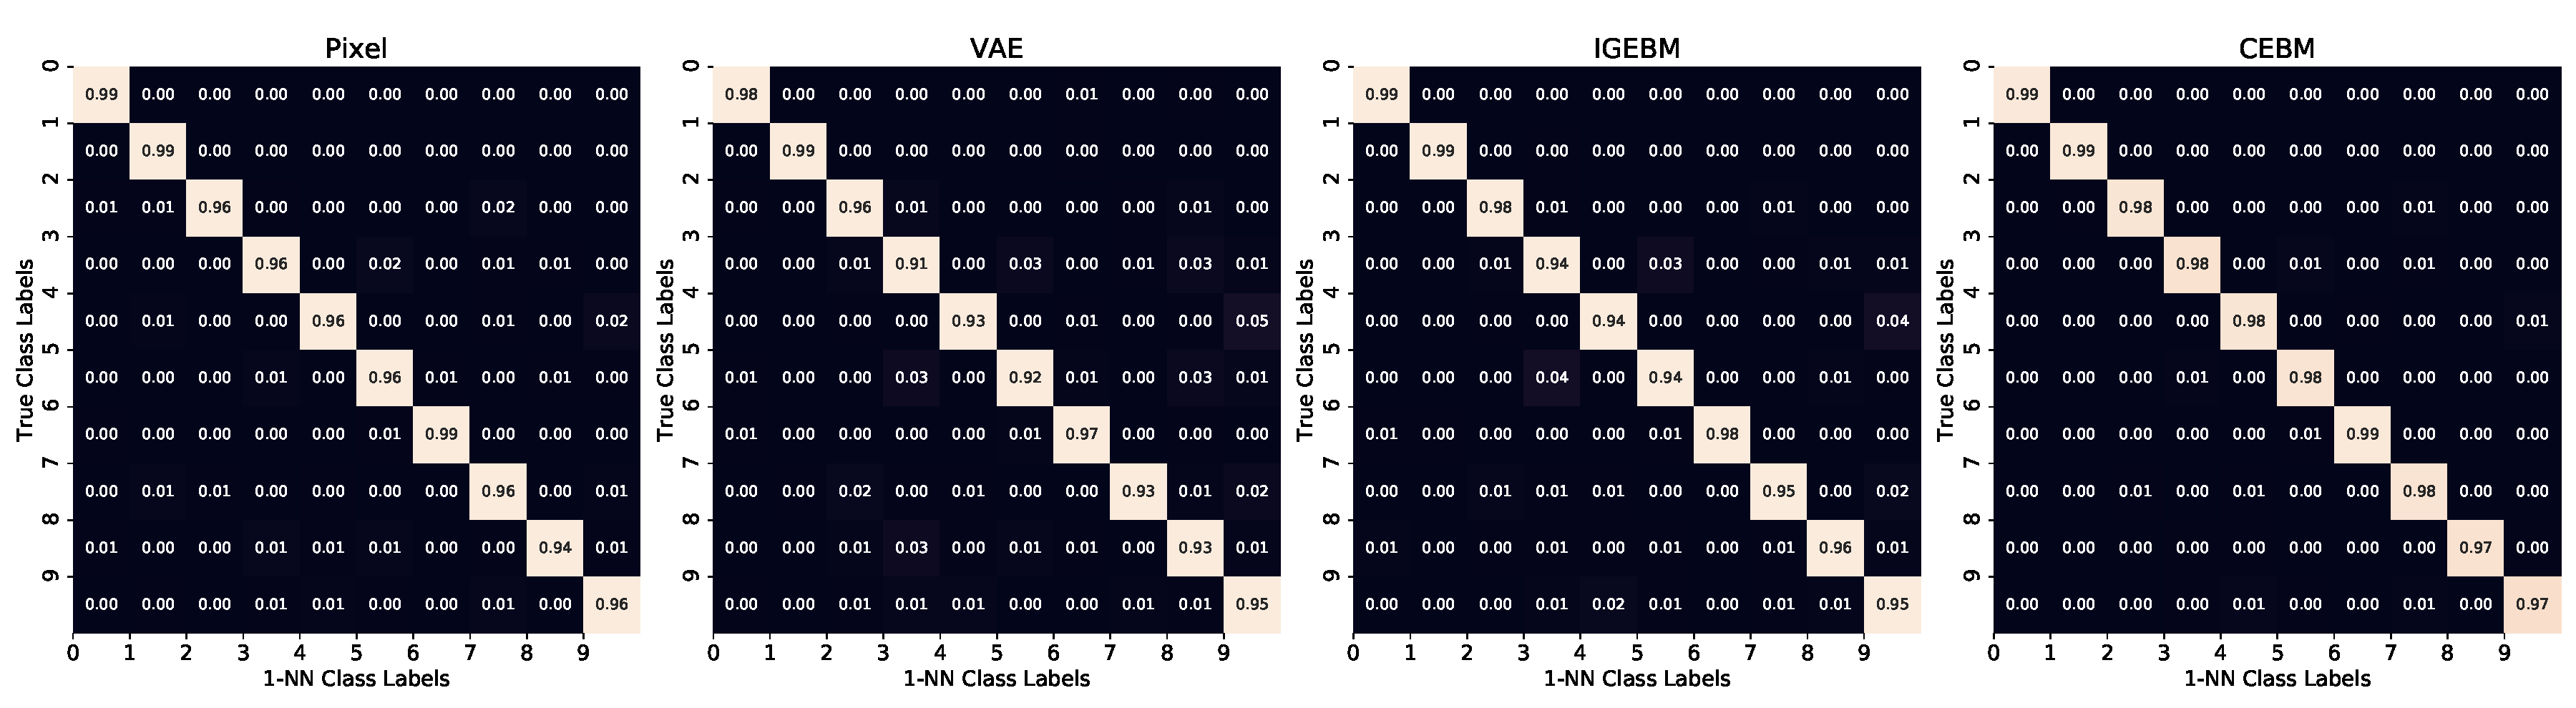
\includegraphics[width=\linewidth]{figures/confusion_matrix_14row_mnist.pdf}
\caption{MNIST}
\label{appendix:confusion-matrices-mnist}
\end{figure}
\begin{figure}[!h]
\centering
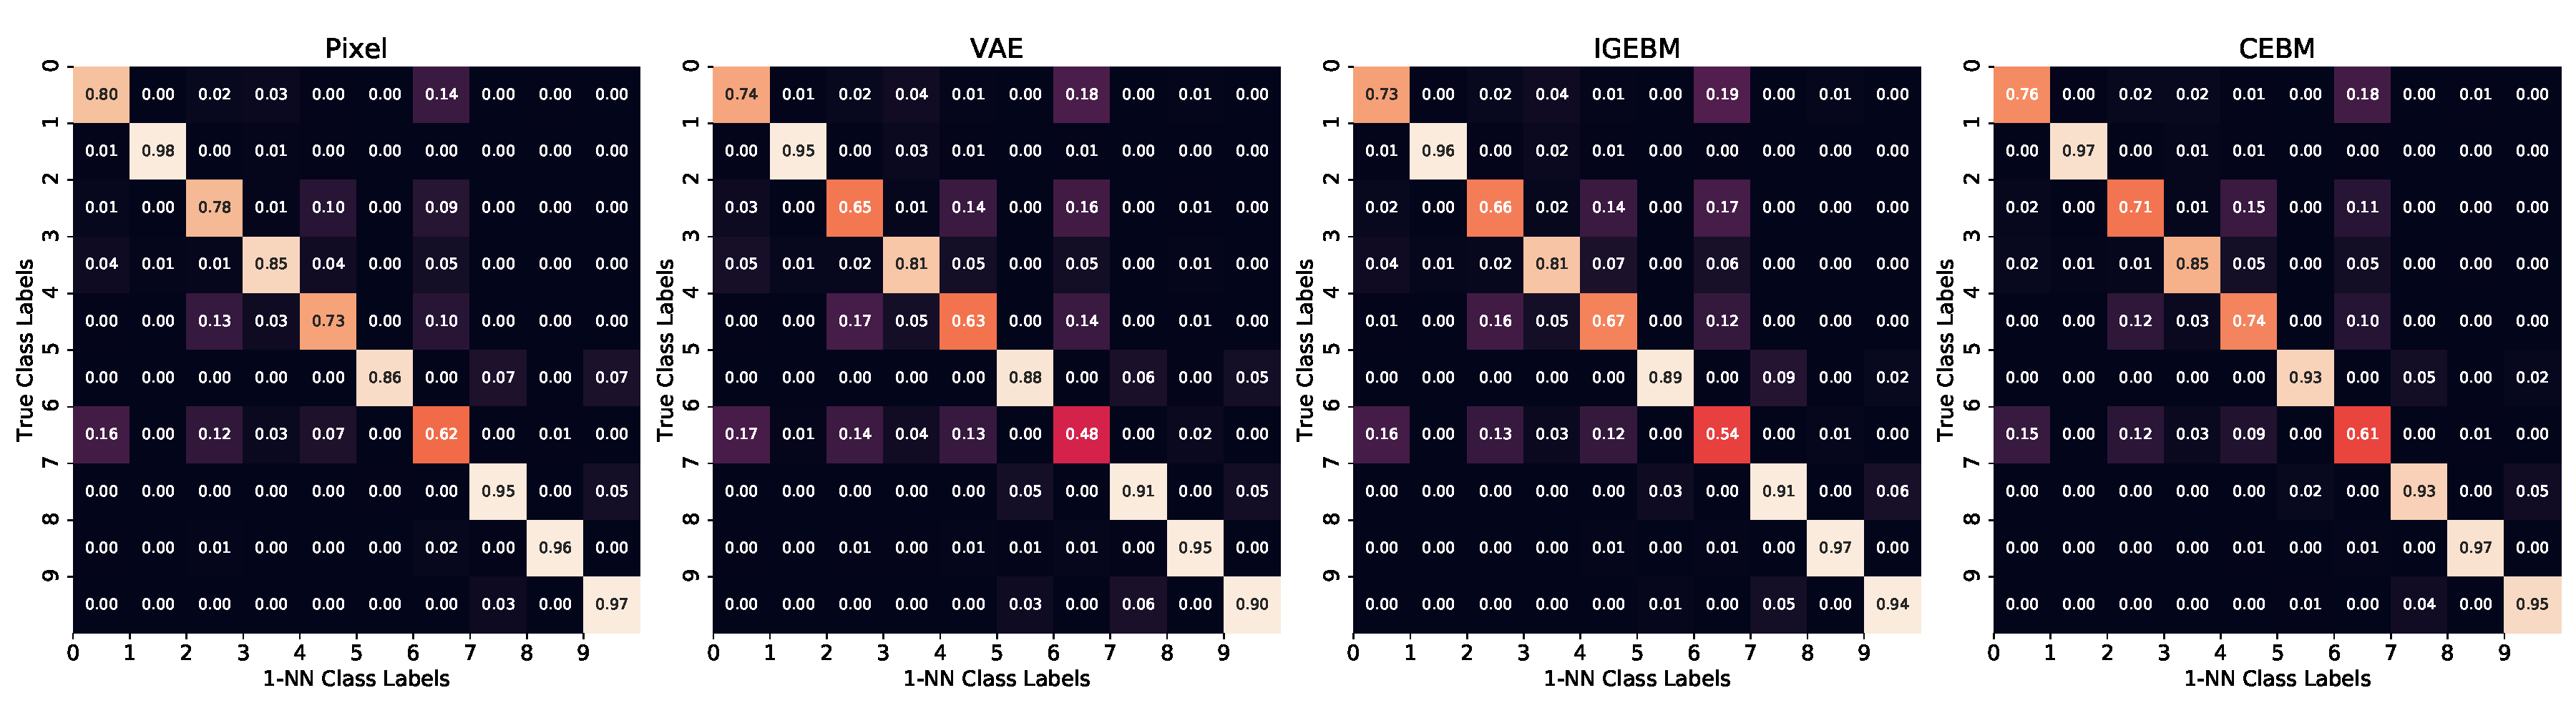
\includegraphics[width=\linewidth]{figures/confusion_matrix_14row_fashionmnist.pdf}
\caption{Fashion-MNIST}
\label{appendix:confusion-matrices-fmnist}
\end{figure}
\vspace{-2em}
\begin{figure}[!h]
\centering
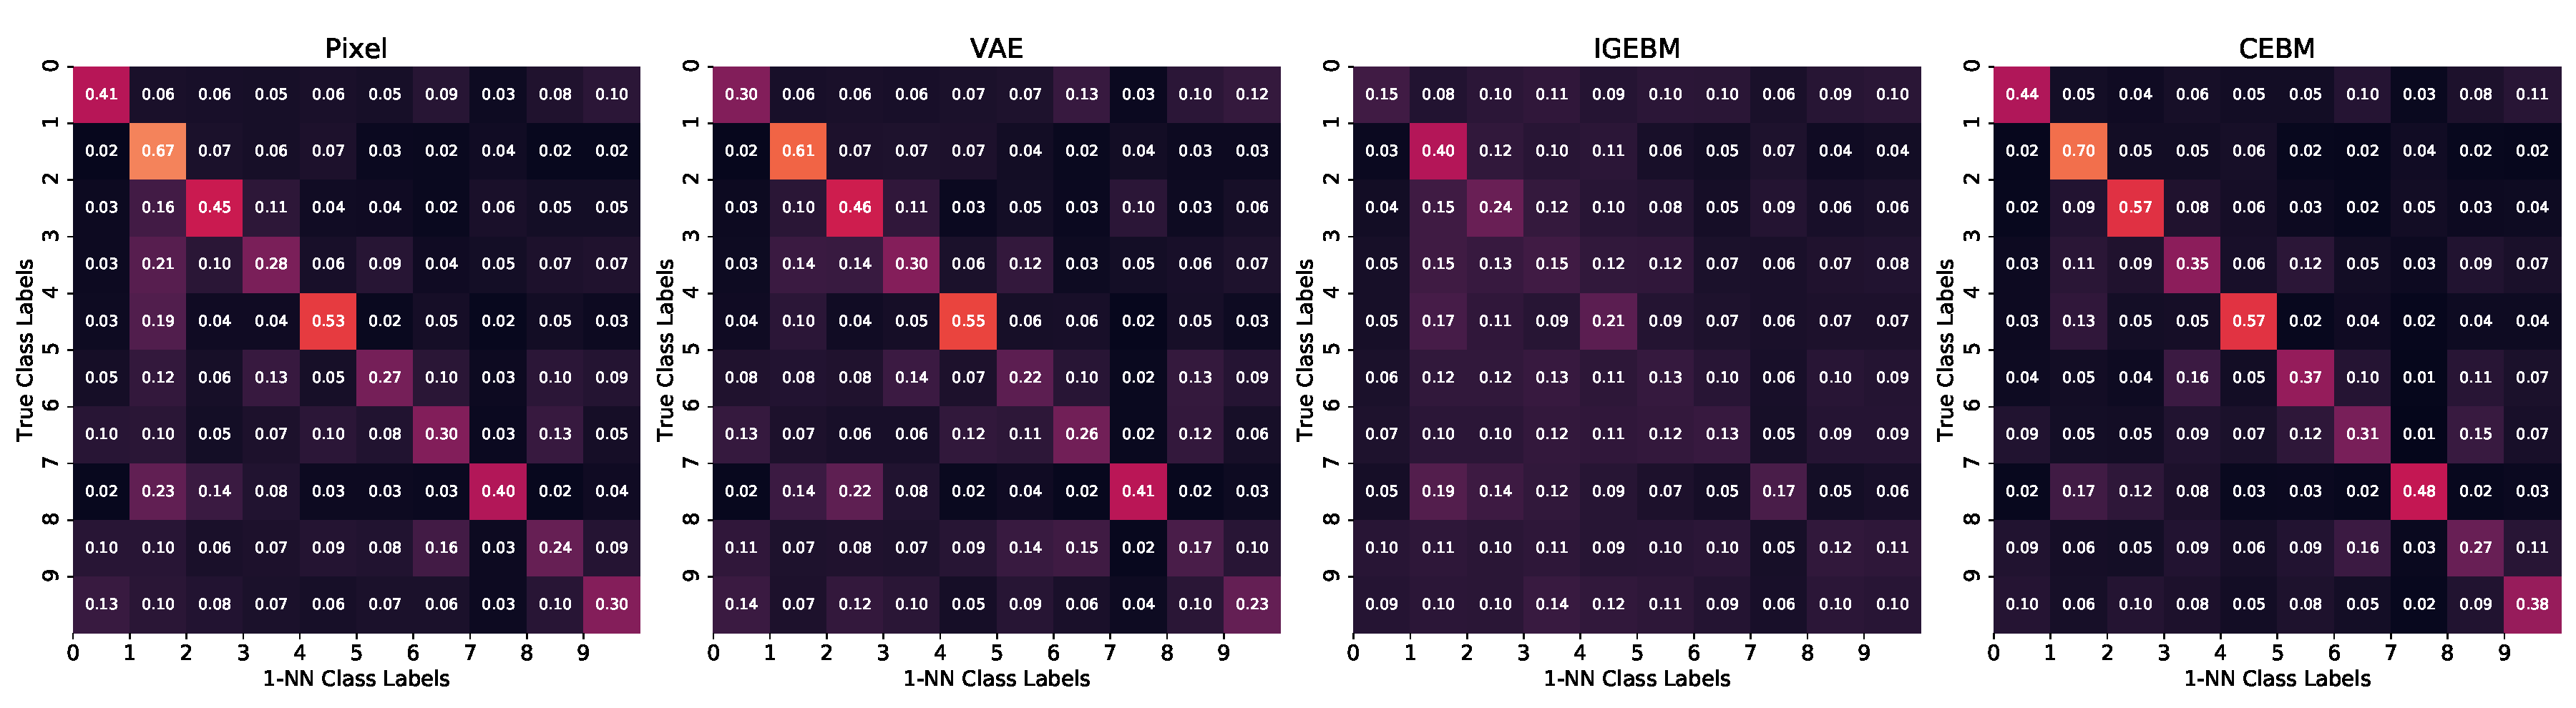
\includegraphics[width=\linewidth]{figures/confusion_matrix_14row_svhn.pdf}
\caption{SVHN}
\label{appendix:confusion-matrices-svhn}
\end{figure}
\vspace{-2em}
\begin{figure}[!h]
\centering
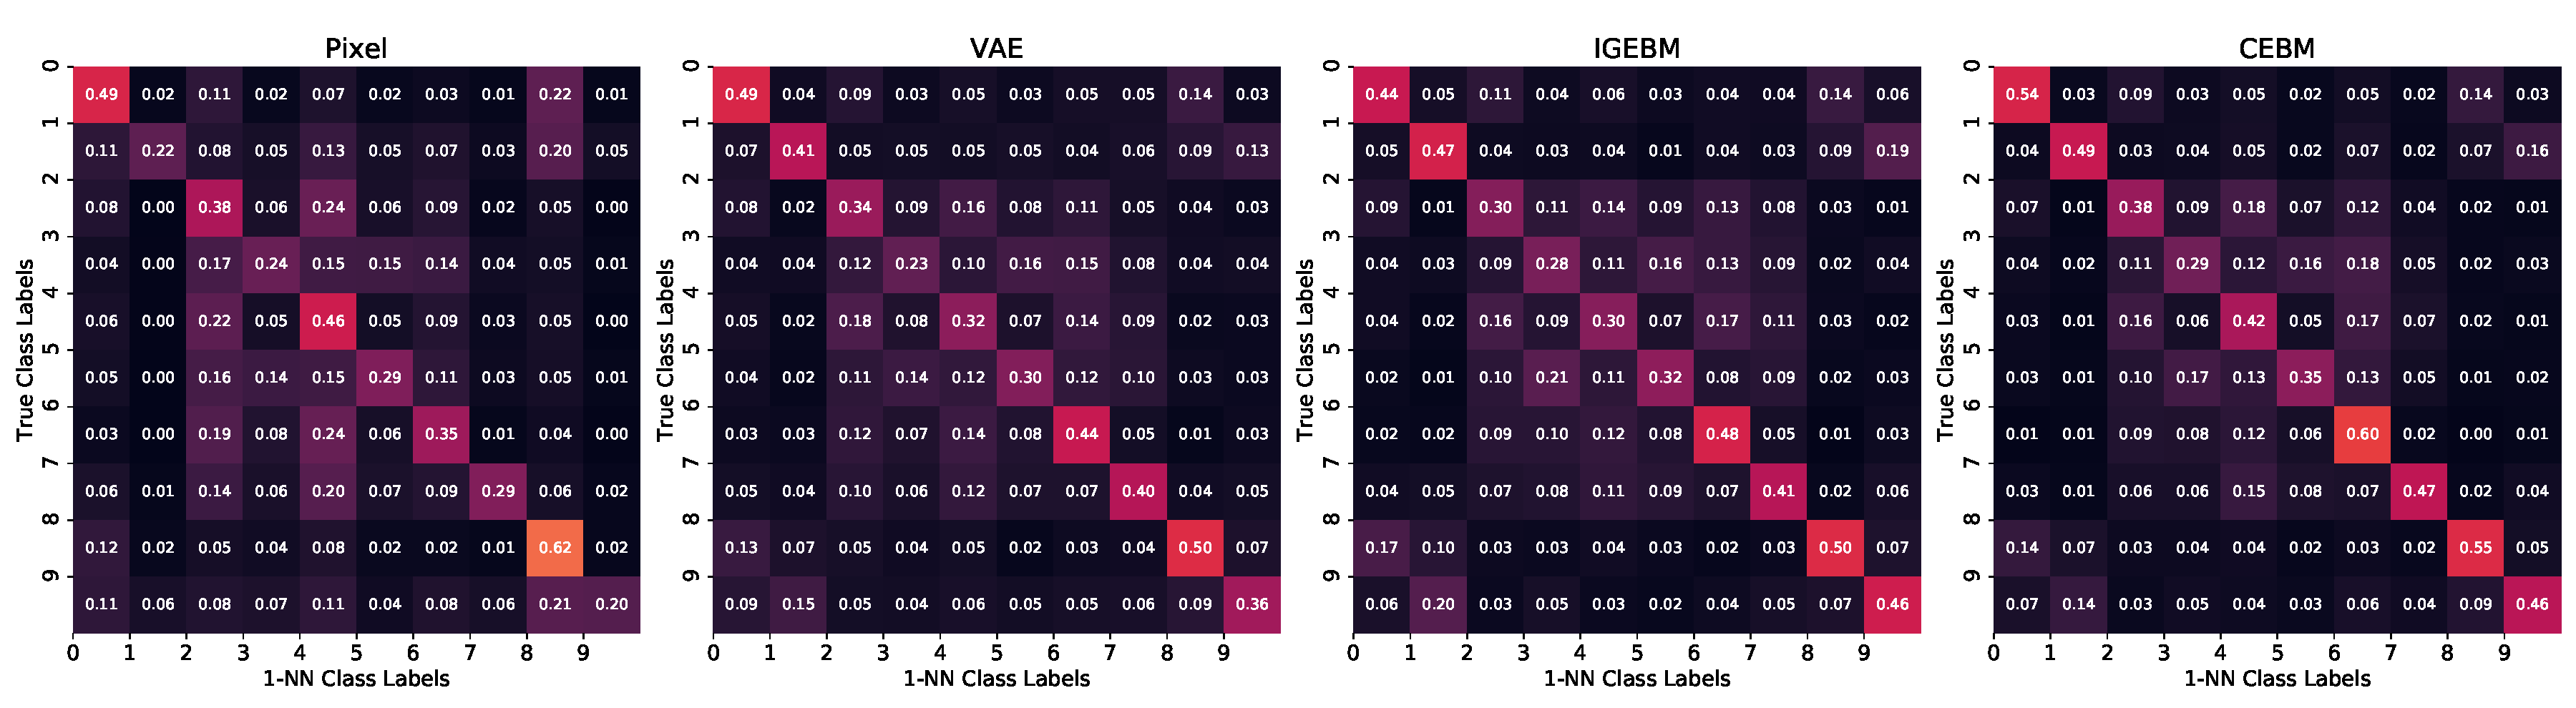
\includegraphics[width=\linewidth]{figures/confusion_matrix_14row_cifar10.pdf}
\caption{CIFAR10}
\label{appendix:confusion-matrices-cifar10}
\end{figure}

\newpage
\subsection{Out-of-Distribution Detection}
\label{appendix-sec:ood-detection}
We compute the AUROC score in OOD detection based on two different score functions.
\setlength{\tabcolsep}{4.5pt}
\begin{table*}[!h]
\caption{AUROC scores in OOD Detection. We use $\log p_{\q}(\x)$ and $\| \nabla_{\x}\log p_{\q}(\x)\|$ as score functions.The left block shows results of the models trained on F-MNIST and tested on MNIST, E-MNIST, Constant (C); The right block shows results of the models trained on CIFAR-10 and tested on SVHN, Texture and Constant (C).}
\centering
\begin{tabular}{l|ccc|ccc||ccc|ccc}
\toprule
& \multicolumn{6}{c||}{Fashion-MNIST} &    \multicolumn{6}{c}{CIFAR-10}\\
& \multicolumn{3}{c|}{$\log p_{\q}(\x)$} & \multicolumn{3}{c||}{$\| \nabla_{\x}\log p_{\q}(\x)\|$} &  \multicolumn{3}{c|}{$\log p_{\q}(\x)$} & \multicolumn{3}{c}{$\| \nabla_{\x}\log p_{\q}(\x)\|$}\\
\midrule
            &  MNIST  & E-MNIST& C &  MNIST & E-MNIST & C &  SVHN & Texture & C &  SVHN & Texture & C \\
\midrule
VAE         & .50 & .39 & .9 & .61 & .57 & .1  & .42 & \textbf{.58} & .41 & .38 & \textbf{.51} & .37 \\
IGEBM       & .35 & .36 & .90 & .78 & .82 & .96& .45 & .31 & .64 & .33 & .17 & \textbf{.62} \\
CEBM        & .37 & .34 & .90 & \textbf{.82} & \textbf{.89} & \textbf{.98} & .47 & .32 & \textbf{.66} & .31 & .17 & .54 \\
CEBMM       & \textbf{.56} & \textbf{.56} & \textbf{.92} & .56 & .80 & .95     & \textbf{.55} & .30 & .62 & \textbf{.40} & .23 & \textbf{.62}  \\
\bottomrule
\end{tabular}
\label{app:tab:ood-detection}
\end{table*}
% \end{document}

% \begin{algorithm}[!t]
% \caption{Persistent Contrastive Divergence}
% \label{alg:cebm}
% \begin{algorithmic}[1]
% \State \textbf{input:} $p_\text{data}(\cdot)$, $\q$, $\alpha$, $T$
% \State $\mathcal{B} \gets \{x_b \sim \mathcal{U} \text{ \textbf{for}}\ b = 1 \ldots \text{buffer-size} \}$
% \While{not converged}
% \State $x \sim p_\text{data}(x)$
% \State $x' \sim \mathcal{B}$ with 95\% probability and $\mathcal{U}$ otherwise
% \For{$t = 1 \ldots T$}
% \State $\epsilon \sim \mathcal{N}(0, \alpha)$
% \State $x' \gets x' - \frac{\alpha}{2} \nabla_{x} E_\q (x') + \epsilon$
% \EndFor
% % \State $\vx^{-} \gets \vx^{-}.\text{detach()} $
% \State $\Delta_{\q} \gets \nabla_{\q} E_{\q}(x) - \nabla_{\q} E_\q(x')$  
% \State $\q \gets \text{Adam}(\q, \Delta_{\q})$
% \State $\mathcal{B}[x'] \gets x'$
% \EndWhile
% \State \textbf{return} $\q$
% \end{algorithmic}
% \end{algorithm}

% \newpage
% \section{ICML New Results}
% \begin{table*}[!h]
% \caption{Classification Accuracy. }
% \centering
% %\vspace*{-1.5ex}
% \begin{tabular}{l|cccc|cccc|cccc|cccc}
% \toprule
%  & \multicolumn{4}{c}{MNIST} & \multicolumn{4}{|c}{Fashion-MNIST} & \multicolumn{4}{|c}{CIFAR-10} & \multicolumn{4}{|c}{SVHN}\\
% Models & $1$ & $10$  & $100$ & $full$ & $1$ & $10$  & $100$ & $full$ & $1$ & $10$  & $100$ & $full$ & $1$ & $10$  & $100$ & $full$ \\
% \midrule
% \midrule
% Classifier & 42 & 79 & 93 & 99 & 46 & 68 & 81 & 90 & 16 & 24 & 39 & 71 & 12 & 19 & 62 & 90\\
% \midrule
% VAE & 42 & 85 & 92 & 95 & 41 & 63 & 72 & 81 & 16 & 22 & 31 & 38 & 13 & 13 & 16 & 36\\
% GMM-VAE & 53 & 86 & 93 & 97 & 49 & 68 & 79 & 84 & 19 & 23 & 33 & 39 & 13 & 14 & 23 & 56  \\
% DCGAN & 9 & 13 & 13 & 14 & 10 & 11 & 16 & 17 & 10 & 11 & 12 & 13 & 9 & 11 & 12 & 20 \\
% BIGAN & - & - & - & - & 51 & 70 & 76 & 81 & 17 & 26 & 36 & 45 & - & - & - & -  \\ 
% \midrule
% IGEBM & 63 & 89 & 95 & 97 & 50 & 70 & 79 & 83 & 16 & 26 & 33 & 42 & 10 & 16 & 35 & 49\\
% CEBM & 67 & 89 & 95 & 97 & 52 & 70 & 77 & 83 & 19 & 30 & 42 & 52 & 12 & 25 & 48 & 70 \\
% CEBMM & 67 & 91 & 97 & 98 & 52 & 71 & 80 & 85 & 16 & 28 & 42 & 51 & 10 & 17 & 39 & 60 \\
% \bottomrule
% \end{tabular}
% \label{tab:few-shot classification-2}
% \end{table*}

\comment{

\begin{table}[!b]
\centering
\caption{Classification results from Semi-supervised objectives trained with 10, 100, 1000, and 5000 labelled examples on MNIST and SVHN.}
\begin{tabular}{c|l|cccc}
\toprule
         Datasets &  Models  &   10      & 100       & 1000      & 5000 \\
\midrule
% \multicolumn{5}{c}{MNIST} \\
\midrule
\multirow{2}{*}{MNIST} & M2 & 75 & 89 & 96 & 97\\
                      & SS-CEBM & 80 & 95 & 98 & 99 \\
\midrule
% \multicolumn{5}{c}{SVHN} \\
\midrule
\multirow{2}{*}{SVHN} & M2 & 21 & 34 & 46 & 55 \\
                      & SS-CEBM & 21 & 33 & 47 & 63 \\
\bottomrule
\end{tabular}
\label{tab:ssl}
\end{table}

\subsection{Semi-Supervised Learning}\label{sec:exp:semi}

In the previous experiment, we evaluated classification performance in a setting where no labels are available during training, and no fine-tuning is performed when training the downstream classifier. As a second experiment, we test whether CEBMs can also improve performance in semi-supervised settings~\cite{kingma2014semisupervised,siddharth2017learning,lin2020improving}, in which a limited number of labels are available during training. To do so, we consider model variants that define a distribution $p_\q(x,y,z)$, in which the label is a latent variable. We then maximize the joint distribution $p_\q(x,y)$ for supervised data and the marginal $p_\q(x)$ for unsupervised data. For further details on this objective, see the Appendix. 
% \begin{equation}
% \E_{p_{\text{data}}(x)}\left[ \log p_{\q}(x)\right] + \E_{p_{\text{data}}(x,y)}\left[ \log p_{\q}(x,y)\right]
% \end{equation}

Inspired by JEM objective~\cite{grathwohl2019your}, we propose a extension of CEBM that models both the data and label. We achieve this we use an encoder $t_\q(x)$ that outputs separate components $t_{\q,z}(x)$ and $t_{\q,y}(x)$ for a continuous variable $z$ and the class label $y$. We then combine this with an inductive bias $b_\q(z,y) = b_\q(z) + b_\q(y)$ in which the bias on $z$ is a spherical Gaussian and the bias on $y$ is a uniform distribution over labels. This yields the energy function
\begin{align*}
E_\q(x,y,z) 
&=
- \big( \lambda_y + t_{\q,y}(x) \big)^\top \eta(y) 
\\ 
&\qquad
- \big( \lambda_z + t_{\q,z}(x) \big)^\top \eta(z) 
 - A(\lambda_y,\lambda_z)
\end{align*}
We refer to this model as the Semi-Supervised CEBM (SS-CEBM). The model is similar to the encoder in M2~\cite{kingma2014semisupervised}, which is the baseline we compare against. We perform experiments on MNIST and SVHN with 10, 100, 1000, and 5000 evenly split labels (see Table~\ref{tab:ssl}), where we observe that SS-CEBM is able to achieve competitive results in semi-supervised learning.  


%When there are labels available, we optimize $p_{\q}(x,y)$ which we achieve by marginalizing over $z$. For the unlabeled data, we marginalize over $y$ in $\gamma_{\q}(x,y)$ and optimize the unnormalized distribution $\gamma_{\q}(x)$. 


% The joint distribution $p_{\q}(x, y, z)$ is the same as Equation~\ref{eq:cebmm-joint}
% \begin{align}
% \frac{1}{K} \exp \{A_{0}(t_{\q}(x) + \lambda) - A_{0}(\lambda)\}\left(\sum_y\exp\{f_{\q}(x)[y]\}\right)
% \end{align}
% \begin{equation}
% \label{eq:ssl-cebm-gxy}
% \frac{1}{K} \exp \{A_{0}(t_{\q}(x) + \lambda) -  A_{0}(\lambda) + f_{\q}(\vx)[y]\}.
% \end{equation}
}

% \bibliography{references}[heading=subbibliography]
% \bibliographystyle{icml2021}